\section{Evaluation}
\label{sec:eval}

% В данном разделе мы представили результаты апробации трех семантик на нескольких примерах.
In this section we present the results of the evaluation of three semantics on a set of examples; the semantics were implemented in \textsc{Haskell} in the form of interpreters.
For evaluation we've chosen two simple programs (list reversing and list sorting) and two more complicated (the ``Hanoi Towers''\footnote{\url{https://en.wikipedia.org/wiki/Tower_of_Hanoi}} solver and the
``Bridge and torch''\footnote{\url{https://en.wikipedia.org/wiki/Bridge_and_torch_problem}} problem solver).
% Для каждой программы мы сделали две версии. Оптимистичная версия --- это программа, в которой мы вручную подобрали оптимальный порядок конъюнктов и пессиместичная версия --- программа с неоптимальным порядком конъюнктов. В последующих диаграммах и таблице указаны средние значения 10 запусков тестов. Также для наивной равномерной конъюнкции мы подобрали количество разверток вручную. Для равномерной конъюнкции, основанной на структурной рекурсии, N было фиксировано и равно 100.
Each program was written in two versions: ``optimistic'' (with the order of important conjuncts set to provide the best performance) and ``pessimistic'' (with the order of important
conjuncts set to provide the worst performance).

All benchmarks were run ten times, and the average time was taken. For the naive fair conjunction we cherry-picked the best value of unfolding bound manually. For the fair conjunction
based on structural recursion the bound was set to 100.

\begin{figure}
\centering
\begin{minipage}{.5\textwidth}
  \centering
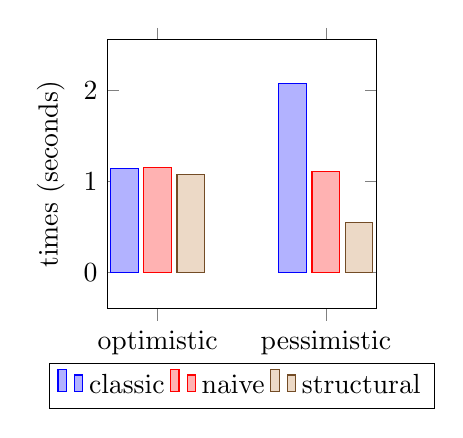
\begin{tikzpicture}
\begin{axis}[
    ybar, ymax = 2, ymin = 0.15,
    enlargelimits=0.3,
    width=5cm, height=5cm,
    legend style={at={(0.5,-0.2)},
      anchor=north,legend columns=-1},
    ylabel={times (seconds)},
    symbolic x coords={optimistic, pessimistic},
    xtick=data
    ]
\addplot coordinates {(optimistic,1.142) (pessimistic,2.073)};
\addplot coordinates {(optimistic,1.151) (pessimistic,1.110)};
\addplot coordinates {(optimistic,1.077) (pessimistic,0.542)};
\legend{classic,naive,structural}
\end{axis}
\end{tikzpicture}
  \captionof{figure}{revers$^o$ evaluation for a list with a length of 90}
  \label{fair:plot-reverso}
\end{minipage}%
\begin{minipage}{.5\textwidth}
  \centering
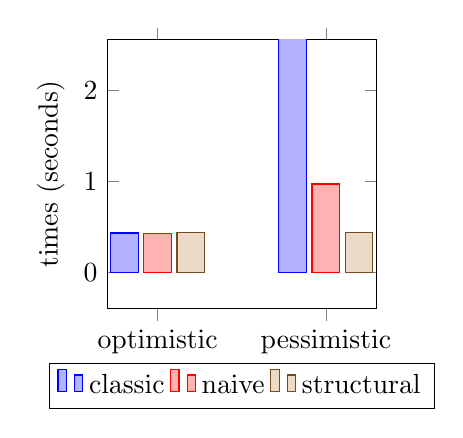
\begin{tikzpicture}
\begin{axis}[
    ybar, ymax = 2, ymin = 0.15,
    enlargelimits=0.3,
    width=5cm, height=5cm,
    legend style={at={(0.5,-0.2)},
      anchor=north,legend columns=-1},
    ylabel={times (seconds)},
    symbolic x coords={optimistic, pessimistic},
    xtick=data
    ]
\addplot coordinates {(optimistic,0.430) (pessimistic,300)};
\addplot coordinates {(optimistic,0.428) (pessimistic,0.969)};
\addplot coordinates {(optimistic,0.433) (pessimistic,0.432)};
\legend{classic,naive,structural}
\end{axis}
\end{tikzpicture}
 \captionof{figure}{sort$^o$ evaluation for a list with a length of 5}
\label{fair:plot-sorto}
\end{minipage}
\end{figure}

\begin{figure}
\centering
\begin{minipage}{.5\textwidth}
  \centering
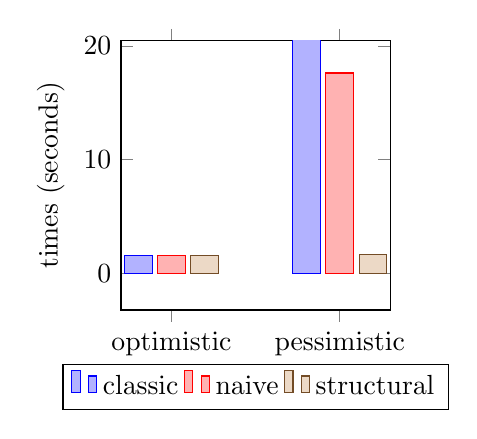
\begin{tikzpicture}
\begin{axis}[
    ybar, ymax = 16, ymin = 1.2,
    enlargelimits=0.3,
    width=5cm, height=5cm,
    legend style={at={(0.5,-0.2)},
      anchor=north,legend columns=-1},
    ylabel={times (seconds)},
    symbolic x coords={optimistic, pessimistic},
    xtick=data
    ]
\addplot coordinates {(optimistic,1.574) (pessimistic,300)};
\addplot coordinates {(optimistic,1.579) (pessimistic,17.604)};
\addplot coordinates {(optimistic,1.585) (pessimistic,1.646)};
\legend{classic,naive,structural}
\end{axis}
\end{tikzpicture}
 \captionof{figure}{``The Tower of Hanoi'' solver evaluation}
\label{fair:plot-hanoi}
\end{minipage}%
\begin{minipage}{.5\textwidth}
  \centering
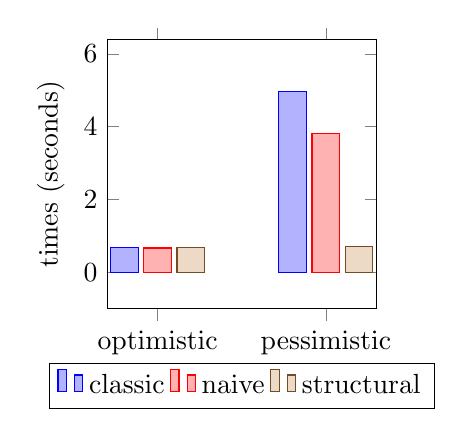
\begin{tikzpicture}
\begin{axis}[
    ybar, ymax = 5, ymin = 0.375,
    enlargelimits=0.3,
    width=5cm, height=5cm,
    legend style={at={(0.5,-0.2)},
      anchor=north,legend columns=-1},
    ylabel={times (seconds)},
    symbolic x coords={optimistic, pessimistic},
    xtick=data
    ]
\addplot coordinates {(optimistic,0.669) (pessimistic,4.956)};
\addplot coordinates {(optimistic,0.663) (pessimistic,3.820)};
\addplot coordinates {(optimistic,0.675) (pessimistic,0.712)};
\legend{classic,naive,structural}
\end{axis}
\end{tikzpicture}
 \captionof{figure}{``Bridge and torch problem'' solver evaluation}
\label{fair:plot-bridge}
\end{minipage}
\end{figure}

% На изображениях 12-15 представлены результаты апробации в виде столбцовых диаграмм. В оптимистичном случае результаты схожи для всех семантик. В пессиместичном случае время работы напрпавленной конъюнкции резко возрастает, время работы наивной равномерной конъюнкции также ворзрастает, но не так сильно. Равномерная конъюнкция, основанная на структурной рекурсии, демострирует схожую эффективность в сравнении с оптимистичным случаем.
Fig.~\ref{fair:plot-reverso}-\ref{fair:plot-bridge} show the results of evaluation in the form of bar charts. In the optimistic case, the results are similar for all semantics.
In the pessimistic case the evaluation time of the directed conjunction rapidly increases, the evaluation time of the naive fair conjunction also increases, but not so much.
The fair conjunction based on structural recursion demonstrates a similar efficiency as in the optimistic case.

% Более подробно результаты представлены на изображении 16. Можно заметить, что время работы программы sorto в пессиместичном случае очень быстро растет с увеличением длины списка для направленной конъюнкции и наивной равномерной. В случае с равномерной конъюнкцией, основанной на структурной рекурсии, пессиместичный случай растет сопостовимо с оптимистичным.
The results are presented in more detail in Fig.~\ref{fair:evaluation-table}. We can conclude that \lstinline{sort$^o$} runtime in the pessimistic case increases
very rapidly with increasing the list length for directed and naive fair conjunctions. In the case of the fair conjunction based on structural recursion the running time in pessimistic case
increases on a par with that in the optimistic one.

\begin{figure}[]
  \small
  \centering
  \begin{tabular}{ c | c | c | c | c | c | c | c }
    \multirow{2}{*}{relation} & \multirow{2}{*}{size} & 
    \multicolumn{2}{c}{directed conjunction} &
    \multicolumn{2}{c}{naive fair conjunction} &
    \multicolumn{2}{c}{structural recursion} \\
    \cline{3-8}
    & & optimistic & pessimistic & optimistic & pessimistic & optimistic & pessimistic  \\ 
    \hline
    \multirow{3}{*}{revers$^o$}
                 & 30   & 0.465 & 0.532 & 0.468 & 0.461  & 0.438 & 0.425 \\
                 & 60   & 0.579 & 0.828 & 0.577 & 0.658  & 0.545 & 0.450 \\
                 & 90   & 1.142 & 2.073 & 1.151 & 1.110  & 1.077 & 0.542 \\
    \hline
    \multirow{5}{*}{sort$^o$}
                 & 3    & 0.418 & 0.432 & 0.420 & 0.420  & 0.424 & 0.425 \\
                 & 4    & 0.424 & 3.924 & 0.424 & 0.455  & 0.429 & 0.429 \\
                 & 5    & 0.430 & >300  & 0.428 & 0.969  & 0.433 & 0.432 \\
                 & 6    & 0.434 & >300  & 0.430 & 11.577 & 0.434 & 0.437 \\
                 & 30   & 1.664 & >300  & 1.636 & >300   & 1.723 & 1.751 \\ 
    \hline
    hanoi$^o$    & -    & 1.574 & >300  & 1.579 & 17.604 & 1.585 & 1.646 \\
    \hline
    bridge$^o$   & -    & 0.669 & 4.956 & 0.663 & 3.820 & 0.675 & 0.712    

  \end{tabular}
  \caption{The results of evaluation: running times of benchmarks in seconds}
  \label{fair:evaluation-table}
\end{figure}

% Подводя итог, равномерная конъюнкция, основанная на структурной рекурсии сопоставима по эффективности с направленной конъюнкцией. Более того, это конъюнкция слабо зависит от порядка конъюнктов.
To summarize, the fair conjunction based on structural recursion does not introduce any essential overhead in comparison with directed conjunction in an optimistic case. At the same time it
weakly depends on the order of the conjuncts, and thus demonstrates much better performance in the pessimistic case.
